\section{Learning from failure}\label{sec:selfmod}

Until this release, every repair of the engine began as a sentence in a log written by hand: the builder stalls here, the filter eats the budget there, so the next version should do something else. The repairs were good ones, and they built most of the parts of Section~\ref{sec:brain}, but the engine could not read them. Release \anaxiaVersion{} turns them into data. An attempt that fails now leaves a record that names what failed, changes one rule of the engine, and is closed only when the next attempt, run under the changed rule, has an outcome of its own. This section describes the records, proves that the loop which writes them always stops, and reads the log of the runs so far.

\subsection{Records and the rule book}\label{ssec:records}

A \emph{rule} is a named setting that a run reads: how the object is written down, which filters are hard, how candidates are generated, which stored results may be used as lemmas, what is searched before an attack, what the budget is, and which modes of work exist. The \emph{rule book} is the current value of every rule, with a version number that rises by one at each change. A \emph{change} names one rule, its kind (one of nine: mode, representation, strategy, library, retrieval, scope, reduction, check, budget), its old value, its new value, and the measurement it is meant to improve.\footnote{A change without that measurement is rejected by the package, and so is a change whose stated old value is not the current one. The first rule makes every change testable: the next attempt either moves the named number or it does not. The second makes the rule book a sequence of edits that can be replayed from version~0.}

An attempt ends in one of four outcomes: \emph{closed}, when the target is settled and the result has passed every check; \emph{partial}, when a weaker statement or a piece of the target has passed; \emph{failed}, when the attempt ran and produced nothing that passed; and \emph{stopped}, when no checkable form of the next step exists under the current rules. A record is written for every attempt. It holds the target, the number of the attempt, the version of the rule book, the outcome, the part of the engine that failed together with the measured evidence, a diagnosis, the change, and the outcome of the retry. The diagnosis is one of nine failure kinds, each the answer to one question: was there no mode that could even state the object, did a hard filter take the budget, did the generator produce only failures, could no rule fire, was the argument found but impossible to arrange as required, was the target already settled, was the statement aimed at too strong, was the computation too large, or was the object searched in a form that hides the property?

\begin{figure*}[t]
\centering
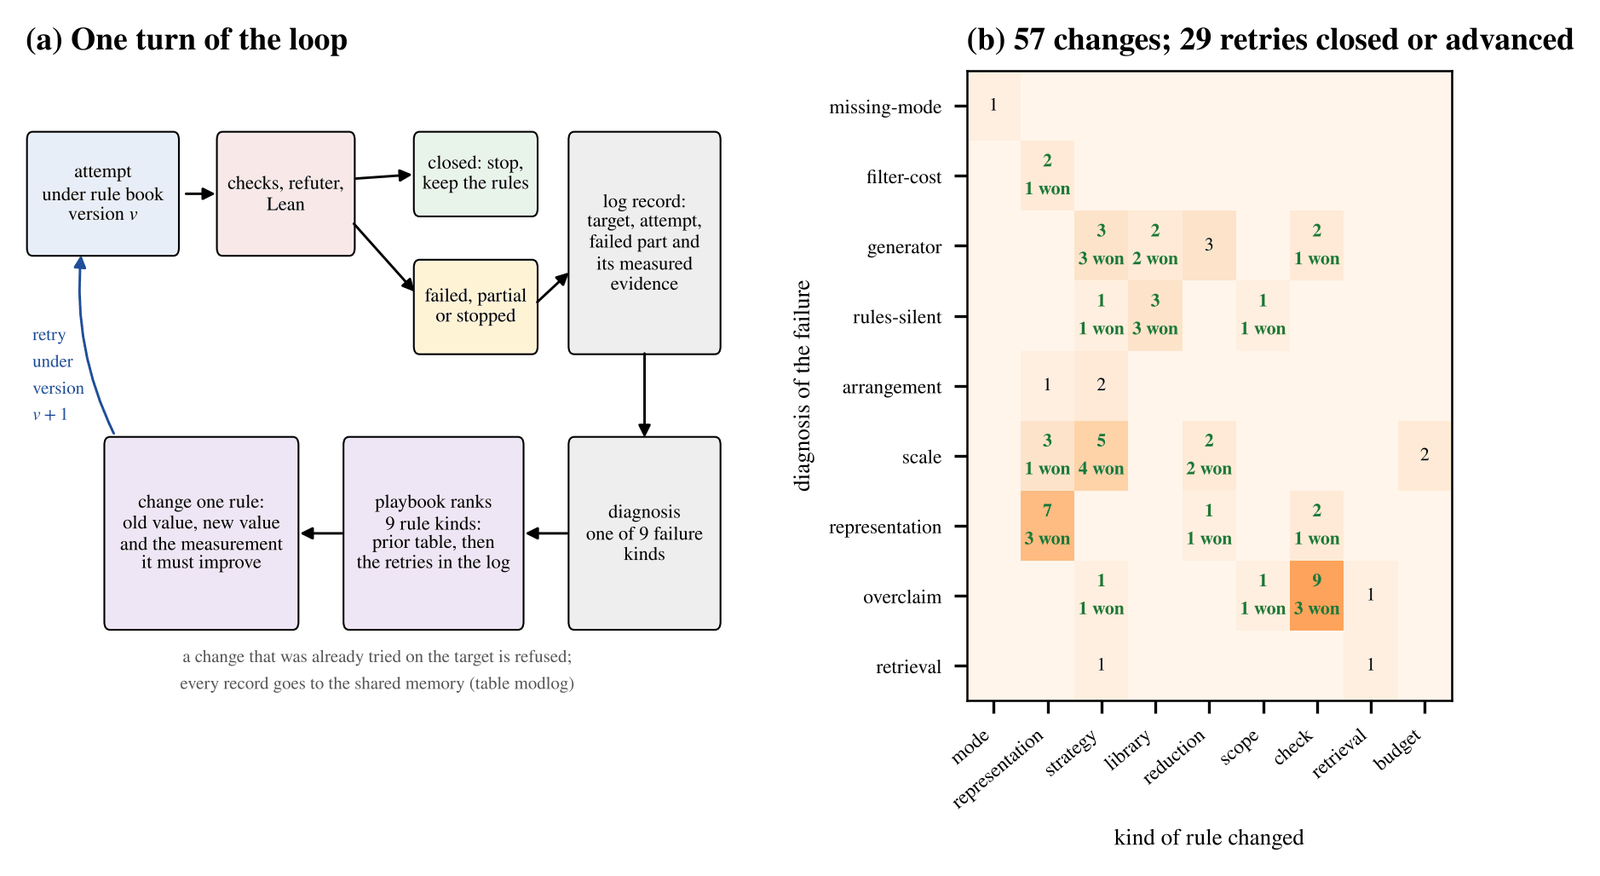
\includegraphics[width=\textwidth]{figures/fig_modloop}
\Description{Left: a flow diagram from an attempt, through the checks, to either a closed result or a failure; a failure goes to a log record, a diagnosis, the playbook, a change of one rule, and a retry under the next version of the rule book. Right: a heat map of failure kinds against kinds of rule changed, with counts and the number of retries that closed or advanced.}
\caption{The learn-from-failure loop. (a) One turn. An attempt runs under version $v$ of the rule book and goes through the checks, the refuter and, where the statement has a Lean form, the kernel. A closed attempt stops the loop and changes nothing. Any other outcome writes a record, the record is diagnosed, the playbook ranks the kinds of rule for that diagnosis (Proposition~\ref{prop:playbook}), one rule is changed, and the retry runs under version $v+1$. (b) Every change of the log so far, by the failure that caused it (rows) and the kind of rule it altered (columns); a cell gives the number of changes and, in green, how many of their retries closed or advanced the target.}
\label{fig:modloop}
\end{figure*}

\subsection{The loop and why it stops}\label{ssec:loop}

The loop is short (Fig.~\ref{fig:modloop}(a)). It makes an attempt under the current rule book. If the attempt closes, the record is written and the loop ends. Otherwise the record is diagnosed, the playbook ranks the nine kinds of rule for that diagnosis, a proposer turns the best-ranked kind that still has a move into one concrete change, the change is applied, and the record is written with it. The next attempt runs under the new rule book, and its outcome is entered as the retry of the record before it. Two guards keep the loop from going round in circles: a change must name the measurement it is meant to improve, and a change already made on the same target, meaning the same rule set to the same value, is refused.

The second guard is enough to make the loop finite, and the bound depends only on what the playbook can propose.

\begin{proposition}\label{prop:loopstops}
Let $C$ be the finite set of changes that the proposer can return for a target. Then the loop makes at most $|C|$ changes and at most $|C|+1$ attempts on that target.
\end{proposition}

\begin{proof}
Every change the loop applies to the target lies in $C$, and no two of them are equal, because a change equal to an earlier one is refused. The applied changes therefore form a list without repetitions whose entries all lie in $C$, and such a list has at most $|C|$ entries: by induction on its length, removing its first entry $c$ from both the list and $C$ leaves a list without repetitions inside $C\setminus\{c\}$, which has one element fewer. Each attempt after the first follows exactly one applied change, since an attempt that is not followed by a change ends the loop, so there are at most $|C|+1$ attempts.
\end{proof}

The proof is formalised in the module \lean{EBLLM.SelfMod} of the engine's Lean library, as the theorems \lean{loop\_changes\_le} and \lean{loop\_attempts\_le}; both depend only on the standard axioms (Appendix~\ref{app:checks}).\footnote{The same counting lemma gives the bound on descents used in Section~\ref{sec:seed}: a strictly monotone sequence of integers inside an interval of length $\ell$ has at most $\ell+1$ terms, so a descent inside it has at most $\ell$ steps. In the package a hard cap of twelve attempts per target sits on top of Proposition~\ref{prop:loopstops}; it has never been reached.}

The ranking is where the log feeds back into the loop. For a diagnosis $d$, the table of the package lists the kinds of rule that usually help, best first, and gives the kind in position $i$ the prior weight $p=1/(2+i)$; a kind not listed gets $p=1/10$. If changes of kind $k$ have been made $t$ times after a failure of kind $d$, and $w$ of their retries closed or advanced the target, the kind is scored by
\begin{equation}\label{eq:playbook}
s(d,k)=\frac{w+2p}{t+2}.
\end{equation}

\begin{proposition}\label{prop:playbook}
The score~\eqref{eq:playbook} is the posterior mean of the success rate of changes of kind $k$ after failures of kind $d$, under the prior $\mathrm{Beta}(2p,\,2-2p)$ and $w$ successes in $t$ independent tries. In particular the prior counts as two tries, its weight in the score is $2/(t+2)$, and as $t\to\infty$ with $w/t\to q$ the score tends to $q$.
\end{proposition}

\begin{proof}
A $\mathrm{Beta}(a,b)$ prior and $w$ successes in $t$ Bernoulli tries give the posterior $\mathrm{Beta}(a+w,\,b+t-w)$, whose mean is $(a+w)/(a+b+t)$. With $a=2p$ and $b=2-2p$ this is $(w+2p)/(t+2)$. Writing it as $\tfrac{2}{t+2}\,p+\tfrac{t}{t+2}\,\tfrac{w}{t}$ shows the weight of the prior and the limit.
\end{proof}

So a fresh engine follows the table, and an engine with a long log follows its own record. A kind that keeps failing on a diagnosis falls below the next one after a few tries: two failed tries take a first choice from $1/2$ to $1/4$, below the untried second choice at $1/3$.

\subsection{What the log shows}\label{ssec:modlogread}

The log bundled with the package holds \modAttempts{} attempts on \modTargets{} targets and \modChanges{} changes of rule (Table~\ref{tab:modlog}, Fig.~\ref{fig:modladder}).\footnote{The records of the construction run were taken from the logs of the runs of 19 October, which give for each attempt its measured evidence and the change that followed, and were written in the format of the loop. The loop of Section~\ref{ssec:loop} produces the same records itself for every new run.} \modBuilt{} of the changes were built and tried; the retries of \modAdvanced{} of them closed their target. The most common kind of change was a change of \modTopKind{} (\modTopKindN{} times): most failures came from searching for an object in a form in which the property it needed was invisible, and the cure was to write the candidates differently, so that a filter held by construction instead of being tested afterwards.

% generated by figures/src/make_tables_round7.py; do not edit
\begin{table*}[t]
\caption{Every rule change in the log of the learn-from-failure loop (file \texttt{modlog.json} of the package). A row is one failed attempt: the target, the attempt, the diagnosis, the rule that was changed with its old and new value, the measurement the change was meant to improve, and the outcome of the retry under the changed rules. Records of attempts that closed carry no change and are not listed.}
\label{tab:modlog}
\centering
\scriptsize
\setlength{\tabcolsep}{3pt}
\begin{tabular}{@{}p{0.15\textwidth}p{0.03\textwidth}p{0.075\textwidth}p{0.43\textwidth}p{0.19\textwidth}p{0.06\textwidth}@{}}
\toprule
\rr Target & \rr Try & \rr Diagnosis & \rr Rule changed: old $\to$ new & \rr Meant to improve & \rr Retry \\
\midrule
\multicolumn{6}{@{}l}{\emph{Construction mode on planar colouring gadgets, 19 October 2026}} \\
\rr Steinberg gadget (k = 5) & \rr 1 & \rr missing-mode & \rr mode: crossing $\to$ crossing and construction (exists-forall SAT over graphs) & \rr a sound 'none found' bound for each number of vertices & \rr failed \\
\rr Steinberg gadget (k = 5) & \rr 2 & \rr filter-cost & \rr representation: lazy Kuratowski cuts $\to$ planar frames: gadgets glued at terminals on one face & \rr share of the budget spent on planarity & \rr failed \\
\rr Steinberg gadget (k = 5) & \rr 3 & \rr generator & \rr strategy: random composition $\to$ goal-directed builder: grow the forcing argument with the graph & \rr tries to a forcer & \rr closed \\
\rr SAT search, profile (3, 3, 4) & \rr 1 & \rr filter-cost & \rr representation: lazy Kuratowski cuts $\to$ 2-page book embedding along a fixed spine & \rr seconds to a 15-vertex gadget & \rr closed \\
\rr level-two gadget (contact distances $\ge$ 4) & \rr 1 & \rr rules-silent & \rr library: forward rules only $\to$ every stored forcer is a lemma rule, applied by case split & \rr contact distances the builder can reach & \rr closed \\
\rr Erd\H{o}s's question, k = 6 & \rr 1 & \rr generator & \rr reduction: a planar graph with no 4-, 5-, 6-cycles that is not 3-colourable $\to$ one gadget: not-all-equal, no 4-, 5-, 6-cycles, contact distances (3, 3, 5) or (5, 5, 3) & \rr size of the object searched & \rr failed \\
\rr Erd\H{o}s's question, k = 6 & \rr 2 & \rr scale & \rr representation: one node per vertex $\to$ compressed search: each proved gadget is one hub node & \rr largest real size reached (about three times) & \rr failed \\
\rr Erd\H{o}s's question, k = 6 & \rr 3 & \rr arrangement & \rr representation: build, then test planarity $\to$ face-aware moves on one face of the current drawing & \rr moves rejected for planarity & \rr failed \\
\rr Erd\H{o}s's question, k = 6 & \rr 4 & \rr arrangement & \rr strategy: face-aware moves $\to$ search over planar arrangements of the forcing argument & \rr arguments that survive the drawing & \rr not yet built \\
\rr Bordeaux conjecture & \rr 1 & \rr generator & \rr reduction: a planar graph with no 5-cycles and no intersecting triangles that is not 3-colourable $\to$ one two-contact not-equal gadget on the edges of K4 & \rr size of the object searched & \rr failed \\
\rr Bordeaux conjecture & \rr 2 & \rr scale & \rr representation: build, then test planarity $\to$ face-aware moves on one face of the current drawing & \rr moves rejected for planarity & \rr failed \\
\rr Bordeaux conjecture & \rr 3 & \rr arrangement & \rr strategy: face-aware moves $\to$ search over planar arrangements of the forcing argument & \rr arguments that survive the drawing & \rr not yet built \\
\rr dijoin conjecture & \rr 1 & \rr retrieval & \rr retrieval: the conjecture's name $\to$ also papers after its date that say they imply it & \rr settled targets caught before an attack & \rr stopped \\
\bottomrule
\end{tabular}
\end{table*}


\begin{figure*}[t]
\centering
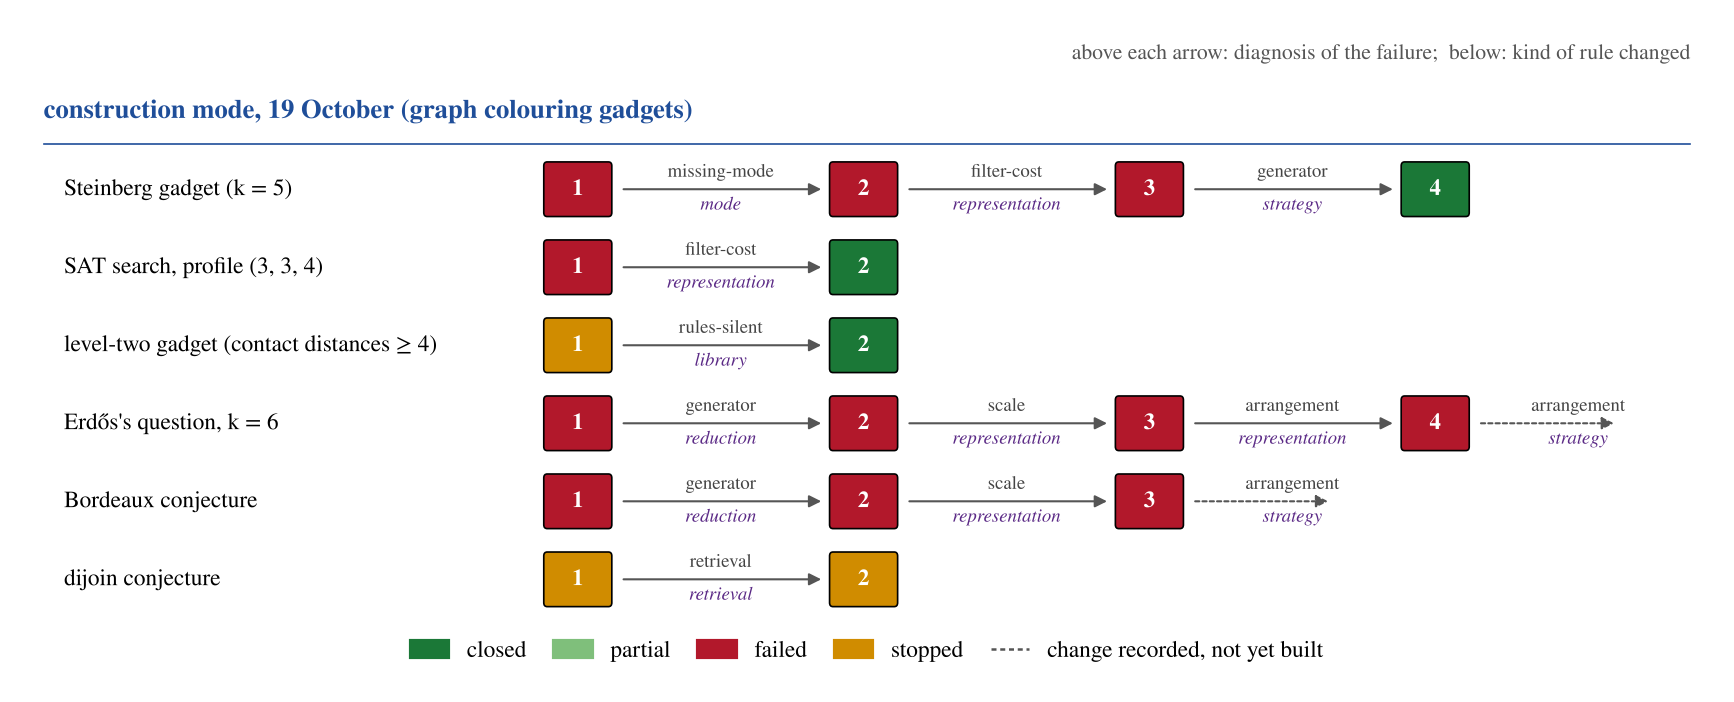
\includegraphics[width=\textwidth]{figures/fig_modladder}
\Description{One row per target. Each attempt is a numbered square coloured by its outcome; the arrows between attempts carry the diagnosis of the failure above and the kind of rule changed below. Dashed arrows are changes recorded and not yet built.}
\caption{Every target of the log as a ladder of attempts. A square is one attempt, coloured by its outcome; above each arrow is the diagnosis of the failure, below it the kind of rule that was changed before the retry. A dashed arrow is a change that has been recorded and not yet built, so its retry has not run.}
\label{fig:modladder}
\end{figure*}

The first target shows the whole loop at work. The task was to rediscover the 15-vertex gadget of Steinberg's counterexample (Section~\ref{ssec:steinberg}). The packaged engine of the time could not even write down a graph, so the first change added a mode of work: construction over graphs, with an exists-forall search. That mode generated planar frames and tested planarity afterwards, and the planarity test took almost every cut, so the second change wrote the candidates as frames glued on one face, planar by construction. The frames were then planar but none forced the colouring, which is a generator failure, and the third change replaced random frames by the goal-directed builder that grows the forcing argument together with the graph. The fourth attempt closed: it found Steinberg's gadget from the rules alone. The second gadget, with all contact distances at least four, was out of reach because no rule could fire from contacts that far apart; one change of library kind, turning every stored gadget into a lemma rule, closed it on the next attempt.

The failures that remain open are as informative. On Erd\H{o}s's question with six colours the engine reduced the target to one gadget, compressed every proved gadget to a single node to cope with the size, and moved to face-aware moves, and each retry failed in the same place: the forcing argument was found, but it could not be laid out with the contacts on one face. The diagnosis became \emph{arrangement} twice in a row, and the change it now calls for, a search over planar arrangements of the forcing argument, is recorded and not yet built. The Bordeaux conjecture followed the same path to the same change. The dijoin conjecture of Chudnovsky, Edwards, Kim, Scott and Seymour \cite{CEKSS16} stopped at once for a different reason: it had already been proved, by a theorem on strong orientations whose paper says that it implies the conjecture \cite{ADN25}, and the first retrieval had missed it.\footnote{The change that followed widened retrieval to the papers after the date of a source that say they imply the target, so that a target settled in this way is caught before an attack starts. The retry found the proof and stopped, as it should.} The loop did not attack it.

The run that crossed a benchmark is the subject of the next section; its records are in the same log, and it went through the same turns: a failure, a diagnosis, one change of rule, a retry under the new rule.
